\documentclass[12pt]{article}
\setlength{\oddsidemargin}{0in}
\setlength{\evensidemargin}{0in}
\setlength{\textwidth}{6.5in}
\setlength{\parindent}{0in}
\setlength{\parskip}{\baselineskip}

\usepackage{amsmath,amsfonts,amssymb,bm,graphics,pgfplots,framed,dsfont,tikz}
\usepackage[scale=0.75,top=1cm,bottom=3cm]{geometry}
\usepackage[dvipsnames]{xcolor}

\begin{document}

\textbf{Minh Anh Nguyen }\\
\textbf{Discrete Mathematics\hfill Assignment-4}

\hrulefill

Section 2.1:

\begin{enumerate}
  \item Consider the following undirected graph.
  \begin{center}
    \includegraphics{img/img-0.png}
  \end{center}
  
        \begin{enumerate}
          \item How many edges are there in this graph?
          \begin{center}
            There are 9 edges in this graph.
          \end{center}
          
        
          \item Give the degree of each vertex.\\
          The dergree of each vertex is:
          \begin{center}
            a has degree 4\\
            b has degree 4\\
            c has degree 2\\
            d has degree 4\\
            e has degree 4\\
          \end{center}

          \item Do these numbers agree with Euler’s first observation? \\
          The sum of the degrees is 4 + 4 + 2 + 4 + 4 = 18. \\
          There are 9 edges in the graph. \\
          The sum of the degrees is doubled the number of edges.\\
          Hence, these numbers agree with Euler's first observation.
        \end{enumerate}

  \item Consider the following directed graph.
        \begin{center}
          \includegraphics{img/img-1.png}
        \end{center}
        \begin{enumerate}
        \newpage
          \item Give the indegree of each vertex.\\
            \begin{center}
              The indegree of a is 1.\\
              The indegree of b is 1.\\
              The indegree of c is 1.\\
              The indegree of d is 2.\\
              The indegree of e is 2.
            \end{center}

          \item Give the outdegree of each vertex.\\
            \begin{center}
              The outdegree of a is 1.\\
              The outdegree of b is 3.\\
              The outdegree of c is 1.\\
              The outdegree of d is 1.\\
              The outdegree of e is 1.
            \end{center}

            \item Compute the sum of the indegrees and the sum of the outdegrees. What do you notice?\\
            The sum of the indegrees is:
            \[1 + 1 + 1 + 2 + 2 = 7\]
            The sum of the outdegrees is:
            \[1+3+1+1+1 = 7\]
            I noticed that the sum of the indegrees is equal to the sum of outdegrees and also equal to the numbers of edges.
            
        \end{enumerate}

  \item A circuit is \textit{simple} if it has no repeated edges. Draw a connected, undirected graph with seven vertices and no simple circuits. How many edges does it have?
  \begin{center}
    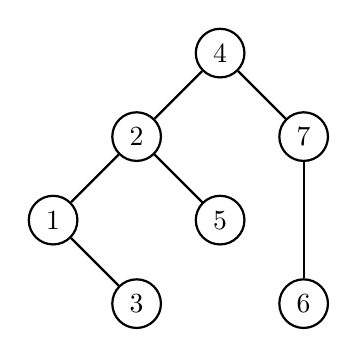
\begin{tikzpicture}[node distance={15mm}, thick, main/.style = {draw, circle}] 
      \node[main] (1) {$1$}; 
      \node[main] (2) [above right of=1] {$2$}; 
      \node[main] (3) [below right of=1] {$3$}; 
      \node[main] (4) [above right of=2] {$4$}; 
      \node[main] (5) [below right of=2] {$5$}; 
      \node[main] (6) [below right of=5] {$6$}; 
      \node[main] (7) [below right of=4] {$7$}; 
      \draw (1) -- (2); 
      \draw (1) -- (3); 
      \draw (2) -- (4); 
      \draw (2) -- (5);
      \draw (7) -- (6);
      \draw (4) -- (7);
      \end{tikzpicture} 
  \end{center}
  It has 6 edges.
  \newpage
  \item Draw an undirected graph with six vertices, each of degree 3, such that the graph is:
  \begin{enumerate}
    \item Connected.
    \begin{center}
      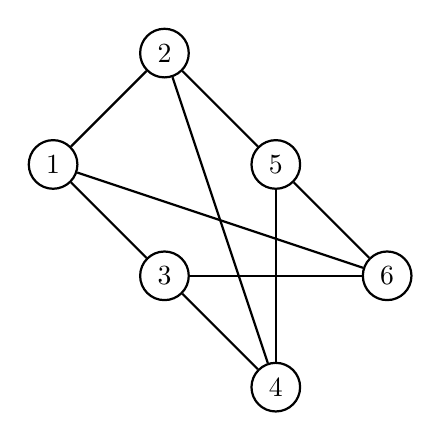
\begin{tikzpicture}[node distance={20mm}, thick, main/.style = {draw, circle}] 
        \node[main] (1) {$1$}; 
        \node[main] (2) [above right of=1] {$2$}; 
        \node[main] (3) [below right of=1] {$3$}; 
        \node[main] (4) [below right of=3] {$4$}; 
        \node[main] (5) [below right of=2] {$5$}; 
        \node[main] (6) [below right of=5] {$6$}; 
        \draw (1) -- (2); 
        \draw (1) -- (3); 
        \draw (3) -- (4);
        \draw (5) -- (4);
        \draw (2) -- (5);
        \draw (1) -- (6);
        \draw (3) -- (6);
        \draw (5) -- (6);
        \draw (4) -- (2);
        \end{tikzpicture} 
    \end{center}
    \item Not connected.
    \begin{center}
      \begin{tikzpicture}[node distance={15mm}, thick, main/.style = {draw, circle}] 
        \node[main] (1) {$1$}; 
        \node[main] (2) [above right of=1] {$2$}; 
        \node[main] (3) [above of=4] {$3$}; 
        \node[main] (4) [below right of=3] {$4$}; 
        \node[main] (5) [below left of=3] {$5$}; 
        \node[main] (6) [below left of=4] {$6$};
        \draw (1) to [out=180,in=270,looseness=5] (1); 
        \draw (2) to [out=0,in=90,looseness=5] (2); 
        \draw (1) -- (2);
        \draw (3) -- (4);
        \draw (3) -- (5);
        \draw (6) -- (5);
        \draw (6) -- (4);
        \draw (6) -- (3);
        \draw (5) -- (4);
        \end{tikzpicture} 
    \end{center}
  \end{enumerate}~\\
  \item A graph is called simple if it has no multiple edges or loops. Draw five different connected, simple, undirected graphs with four vertices.\\
  1.
  \begin{center}
    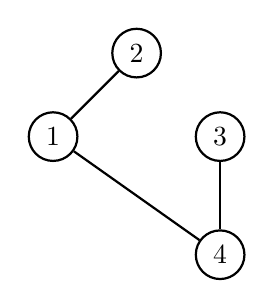
\begin{tikzpicture}[node distance={15mm}, thick, main/.style = {draw, circle}] 
      \node[main] (1) {$1$}; 
      \node[main] (2) [above right of=1] {$2$}; 
      \node[main] (3) [below right of=2] {$3$}; 
      \node[main] (4) [below of=3] {$4$}; 
      \draw (1) -- (2);
      \draw (1) -- (4);
      \draw (3) -- (4);
      \end{tikzpicture} 
  \end{center}
  \newpage
  2.
  \begin{center}
    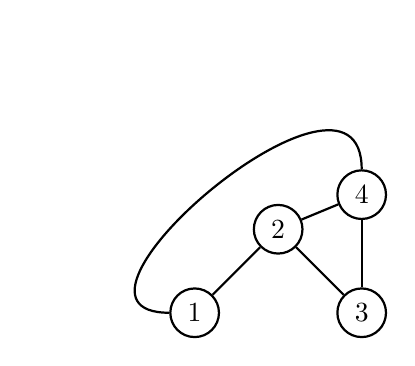
\begin{tikzpicture}[node distance={15mm}, thick, main/.style = {draw, circle}] 
      \node[main] (1) {$1$}; 
      \node[main] (2) [above right of=1] {$2$}; 
      \node[main] (3) [below right of=2] {$3$}; 
      \node[main] (4) [above of=3] {$4$}; 
      \draw (1) -- (2);
      \draw (3) -- (4);
      \draw (2) -- (3);
      \draw (2) -- (4);
      \draw (1) to [out=180,in=90,looseness=1.5] (4);
      \end{tikzpicture} 
  \end{center}
  3.
  \begin{center}
    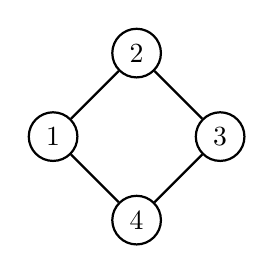
\begin{tikzpicture}[node distance={15mm}, thick, main/.style = {draw, circle}] 
      \node[main] (1) {$1$}; 
      \node[main] (2) [above right of=1] {$2$}; 
      \node[main] (3) [below right of=2] {$3$}; 
      \node[main] (4) [below right of=1] {$4$}; 
      \draw (1) -- (2);
      \draw (2) -- (3);
      \draw (3) -- (4);
      \draw (1) -- (4);
      \end{tikzpicture} 
  \end{center}
  4.
  \begin{center}
    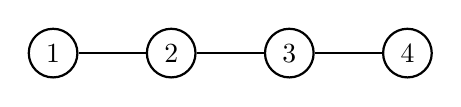
\begin{tikzpicture}[node distance={15mm}, thick, main/.style = {draw, circle}] 
      \node[main] (1) {$1$}; 
      \node[main] (2) [right of=1] {$2$}; 
      \node[main] (3) [right of=2] {$3$}; 
      \node[main] (4) [right of=3] {$4$}; 
      \draw (1) -- (2);
      \draw (2) -- (3);
      \draw (3) -- (4);
      \end{tikzpicture} 
  \end{center}
  5.
  \begin{center}
    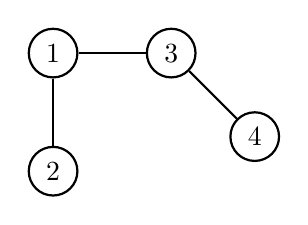
\begin{tikzpicture}[node distance={15mm}, thick, main/.style = {draw, circle}] 
      \node[main] (1) {$1$}; 
      \node[main] (2) [below of=1] {$2$}; 
      \node[main] (3) [right of=1] {$3$}; 
      \node[main] (4) [below right of=3] {$4$}; 
      \draw (1) -- (2);
      \draw (1) -- (3);
      \draw (3) -- (4);
      \end{tikzpicture} 
  \end{center}
  \item An undirected graph is called \textit{complete} if every vertex shares an edge with every other vertex. Draw a complete graph on five vertices. How many edges does it have?\\
  \begin{center}
    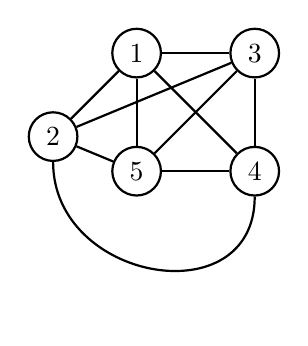
\begin{tikzpicture}[node distance={15mm}, thick, main/.style = {draw, circle}] 
      \node[main] (1) {$1$}; 
      \node[main] (2) [below left of=1] {$2$}; 
      \node[main] (3) [right of=1] {$3$}; 
      \node[main] (4) [below of=3] {$4$}; 
      \node[main] (5) [below of=1] {$5$}; 
      \draw (1) -- (2);
      \draw (1) -- (3);
      \draw (3) -- (4);
      \draw (2) -- (5);
      \draw (2) to [out=270, in=270, looseness=1.5] (4);      
      \draw (4) -- (5);
      \draw (1) -- (4);
      \draw (1) -- (5);
      \draw (2) -- (3);
      \draw (5) -- (3);
      \end{tikzpicture} 
  \end{center}
  It has 10 edges.
\end{enumerate}

\newpage
  Section 2.2:
\begin{enumerate}
  \item Draw Venn diagrams to illustrate De Morgan’s laws for sets (Theorem 2.1).\\~\\
    1. $(A \cup B)' =  A' \cap B'$
    \begin{center}
      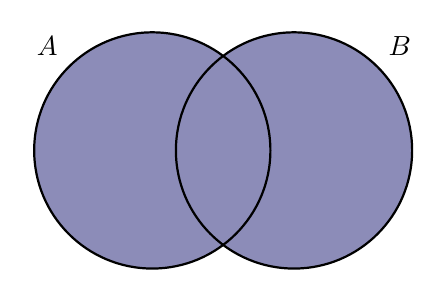
\begin{tikzpicture}[thick,
        set/.style = {circle,
          minimum size = 3cm,
          fill=MidnightBlue!50}]
      
      % Set A
      \node[set,label={135:$A$}] (A) at (0,0) {};
      
      % Set B
      \node[set,label={45:$B$}] (B) at (1.8,0) {};
      

      
      \begin{scope}
        \clip (0,0) circle(1.5cm);
        \clip (1.8,0) circle(1.5cm);
      \end{scope}
      
      \draw (0,0) circle(1.5cm);
      \draw (1.8,0) circle(1.5cm);
            
      \end{tikzpicture}
    \end{center}
\end{enumerate}

\end{document}